%%%%%%%%%%%%%%%%%%%%%%%%%%%%%%%%%%%%%%%%%%%%%%%%%%%%%%%%%%%%%%%%%%%%
% Ergebnisse
%%%%%%%%%%%%%%%%%%%%%%%%%%%%%%%%%%%%%%%%%%%%%%%%%%%%%%%%%%%%%%%%%%%%
\chapter{Results}
  \label{results}

% \todo{
% In this chapter which also could be more than one chapter, depending on the nature of the thesis, the results of the thesis are presented.
% Make sure you illustrate your results with appropriate figures and tables, but do not discuss the results here. This should be done in a separate discussion chapter.
% Or maybe do combine results and discussion and split by research questions.
% }
\todo[inline]{
  Incorporate Nicole's feedback! (see slack DMs)
}

\section{Rule-Based Controller}
- How does it perform?
- On how many days does it needlessly fill the battery?

\section{Discretization}
\begin{figure}[h]
  \centering
  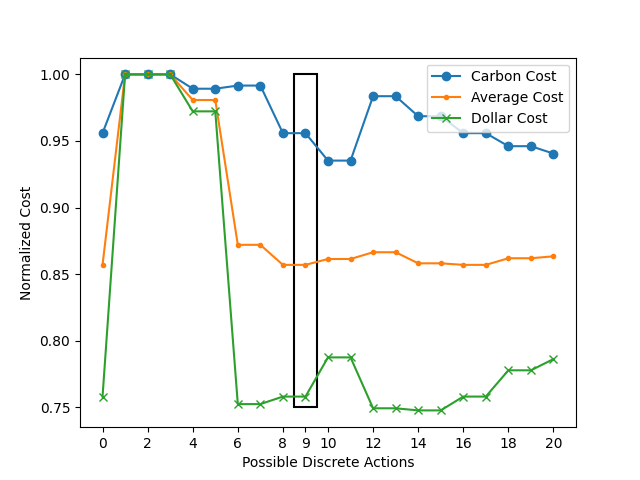
\includegraphics[width=\figurewidth]{figures/discretization.png}
  \caption{This graph shows the effect of the discretization resolution on the rule-based control algorithm. The coarsest resolution that does not significantly impact performance and includes the zero action is 9. In this graph, 0 possible actions means no discretization is applied.}
  \label{fig:discretization}
\end{figure}

In the pre-experiment on the effect of discretization, the rule-based agent performs comparably to the continuous case when discretization resolution is high, and worse on coarse resolutions. The coarsest resolution that performs similarly well as the continuous case is the subdivision into 8 or 9 possible actions.




\section{Hyperparameter Tuning}
\todo{
- How much computational power did the tuning take?
  - if I can find it. If not, just omit.
}
All 200 runs of $\epsilon$-greedy DQN completed successfully.
10/100 runs of UA-DQN, all runs with a batch size of 1, failed.
18/200 runs of DQN-softmax failed, all of which share a batch size of 8.
However, 17 other runs with a batch size of 8 completed successfully.

Table \ref{tab:hyperparameters} shows the results of the tuning process for each algorithm.
For each algorithm, the learning rate had the most significant correlation with final performance, followed by the batch size and the target network update frequency.
The $\epsilon$ parameter of the optimizer Adam showed a large effect only for $\epsilon$-greedy DQN.

Figure \ref{fig:tuning_results} shows a histogram of the final performance of all successful tuning runs.
Both DQN algorithms show a peak at around -5000, which corresponds to strategies that make no or very little use of the battery.
The UA-DQN algorithm learns a superior strategy for more hyperparameters.

\begin{table}[h]
  \centering
  \caption{This Table shows the correlation between tuned hyperparameters and algorithm performance for successful runs.}
  \label{tab:hyperparameters}
  \begin{tabular}{c||c|c|c}
    Algorithm & Hyperparameter & Value for Best Run & \makecell{Correlation with \\ final score} \\ \hline
    UA-DQN & Learning Rate                                & 3e-4 & \bf{-0.47}\\
           & Batch Size                                   & 128 &  0.28\\
           & Adam's $\epsilon$                            & 1e-07 & -0.03\\
           & \makecell{Target Network \\ Update Frequency}& 4 & -0.11\\ \hline
    DQN-softmax & Learning Rate                                 & 3e-4 & \bf{-0.36} \\
                & Batch Size                                    & 128 & -0.18\\
                & Adam's $\epsilon$                             & 1e-05 & -0.02\\
                & \makecell{Target Network \\ Update Frequency} & 4 &  0.16\\ \hline
    DQN-$\epsilon$-greedy & Learning Rate                       & 7e-05 & \bf{-0.33}\\
                & Batch Size                                    & 4 & -0.19\\
                & Adam's $\epsilon$                             & 1e-08 &  0.10\\
                & \makecell{Target Network \\ Update Frequency} & 16 &  0.14

  \end{tabular}
\end{table}



\begin{figure}
  \centering
  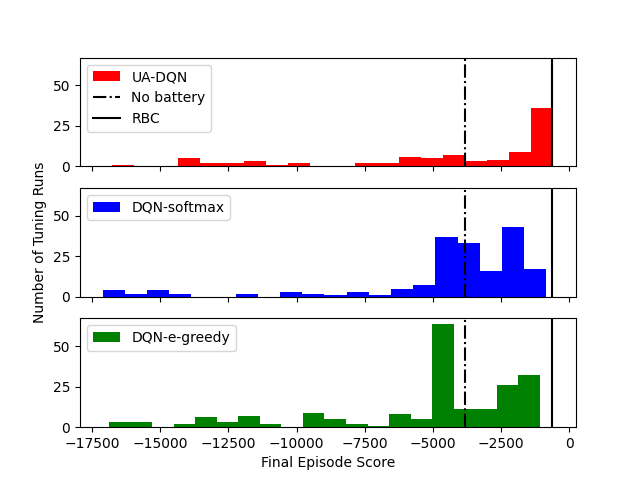
\includegraphics[width=\figurewidth]{figures/tuning_results.png}
  \caption{This histogram shows the final episode reward of all successful tuning runs.}
  \label{fig:tuning_results}
\end{figure}

\section{Comparison of Tuned Algorithms}
Figure \ref{fig:tuning_validation} shows the episode rewards of the selected hyperparameters for each algorithm during training.
Tuned UA-DQN converges faster than the other algorithms, and it converges to a better mean performance, as stated in table \ref{tab:tuned_results}. The hand-engineered rule-based agent outperforms the tuned reinforcement learning algorithms on both metrics.

When repeated with 10 different seeds, a single run of DQN-softmax failed, compared to no failures from the other algorithms.


\begin{figure}
  \centering
  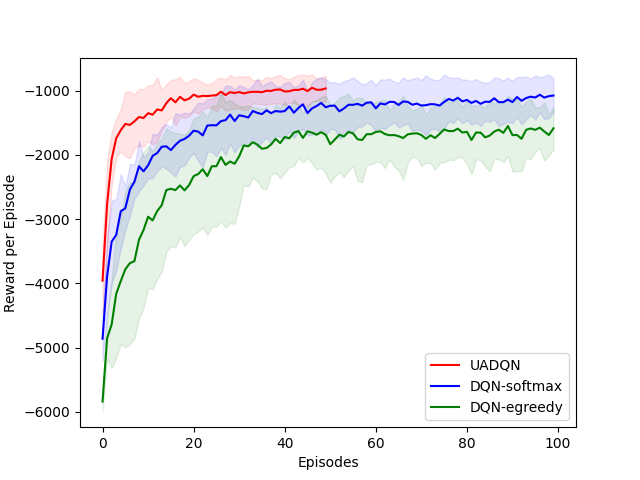
\includegraphics[width=\figurewidth]{figures/tuning_validation.png}
  \caption{This graphic shows the performance during training of the three tuned algorithms. The shaded area shows the standard deviation over 10 runs with different random seeds. Tuned UA-DQN converges after fewer episodes than either DQN variant. UA-DQN was only trained for 50 episodes due to the added computational complexity of the algorithm.}
  \label{fig:tuning_validation}
\end{figure}

\begin{table}
  \centering
  \caption{This table shows the mean performance of tuned algorithms when evaluated using their respective action selection policy for one episode on Building 1.}
  \label{tab:tuned_results}
  \begin{tabular}{l|ccccc}
    Agent                 & Dollar Cost & Carbon Emission & Average \\ \hline
    Control (No Action)   & 1    & 1    & \textbf{1}    \\
    DQN-Softmax           & 0.83 & 0.93 & \textbf{0.88} \\
    DQN $\epsilon$-greedy & 0.82 & 0.93 & \textbf{0.88} \\
    UA-DQN                & 0.82 & 0.91 & \textbf{0.87} \\
    Discrete Rule-Based   & 0.80 & 0.88 & \textbf{0.84}
  \end{tabular}
\end{table}

\begin{figure}
  \centering
  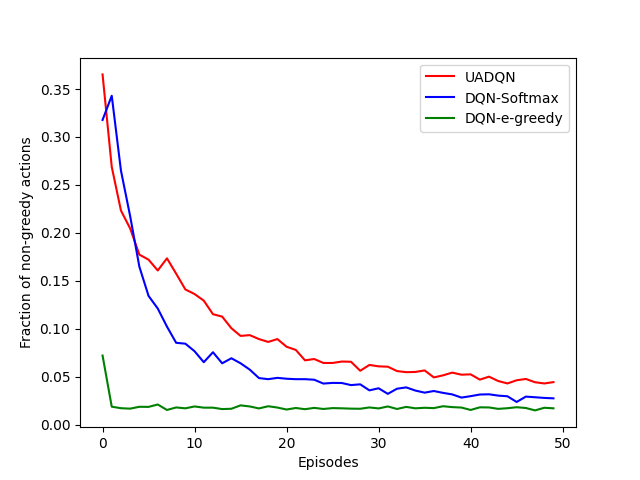
\includegraphics[width=\figurewidth]{figures/non-greedy-fraction.png}
  \caption{This graphic shows the fraction of selected actions that do not correspond to the highest expected value. It highlights the different action selection strategies employed by the different algorithms. UA-DQN keeps exploring for longer than the other strategies.}
  \label{fig:non_greedy_fraction}
\end{figure}

To illustrate the difference in exploration between the algorithms, figure \ref{fig:non_greedy_fraction} shows the fraction of selected non-greedy actions per episode.
All algorithms start out exploring more and then gradually decrease their exploration rate.
DQN-softmax and UA-DQN explore more than $\epsilon$-greedy DQN, which quickly reaches an exploration rate of $\epsilon = 0.02$.
UA-DQN keeps exploring more than the other algorithms.

\clearpage
